%!TEX root = ../report.tex

\begin{document}
	\let\cleardoublepage\clearpage
\chapter{Implementation} \label{sec:implementation}
This chapter briefly describes the implementation of the mediator component, tools involved in the mediator and their purpose, and the strategy followed to collect sensor observation data from different robots over the mediator. 

	\section{Mediator design process}
	The mediator component is a complex and giant piece of software component comprises of various sub-components in it. Before start developing a software component, there are many standards and approaches have been defined in software engineering domain that should be followed by developers to achieve stable development process and at the end finish the project with a successful working product. Since this research work implements a software component, we decided to take up two well-known software development models called Feature driven development from Agile and Component Assembly Model. It is a heterogeneous development model as we take the useful features from two different models.
	
	Feature driven development was first introduced by the book "Java Modeling in Color with UML" \cite{misc15} and first used for a huge bank project. The core concept of FDD is initially developing an overall model and define all possible required features as a list. The overall model for this research work is, a mediator component operates between multiple database instances which runs in a centralized server or in the robot itself. Now the possible feature list for our mediator component is, 
	
	\begin{itemize}
		\item Finding the entities and define their attributes.
		\item Finding a suitable data structure which supports context.
		\item Schema registration for a new task, robots, and sensors.
		\item Creation of observation buckets and update GraphQL type definitions.
		\item Update GraphQL mutations and queries.
	\end{itemize}
	
	
	
	Once the overall model and feature list are defined, we decompose the feature into smaller reusable components. These components are developed individually and combined later back to a single feature on the basis of Component Assembly model. For each feature in the list, a planning schedule is assigned to keep track of time and finish developing the feature on time. Before start implementing a feature, proper design is made to avoid changes in the mediator component in the future. After preparing the plan and design, the next step is building smaller components which form the individual feature. The complete process is repeated until the final mediator component meets the proposed mediator requirements. 
	
	After each release, the mediator is cross verified with the user story and tested on real use cases which are described in the later section [TBD]. Feedbacks are received from the user and improved the mediator stability and reliability on each version which is released on every week.
	
	
	\section{Architecture} 
	This section gives a brief overview of the mediator architecture and the components involved in it.
	The overall architecture is divided into three major sections, Producer or Consumer, Mediator, Data sources.
	

	\subsection{Producer/Consumer}
	
	The leftmost section in figure \ref{fig:architecture} includes any robots or tools which consumes the data from data sources or produces data to the data sources via the mediator component. In the research work, we are not investing the types of consumer/producer involved in the process since the mediator component is being developed to solve general heterogeneous data sources problem with a global audience in mind.
	
	\newpage
	
	\begin{figure}[!htbp] 
		\begin{center}
			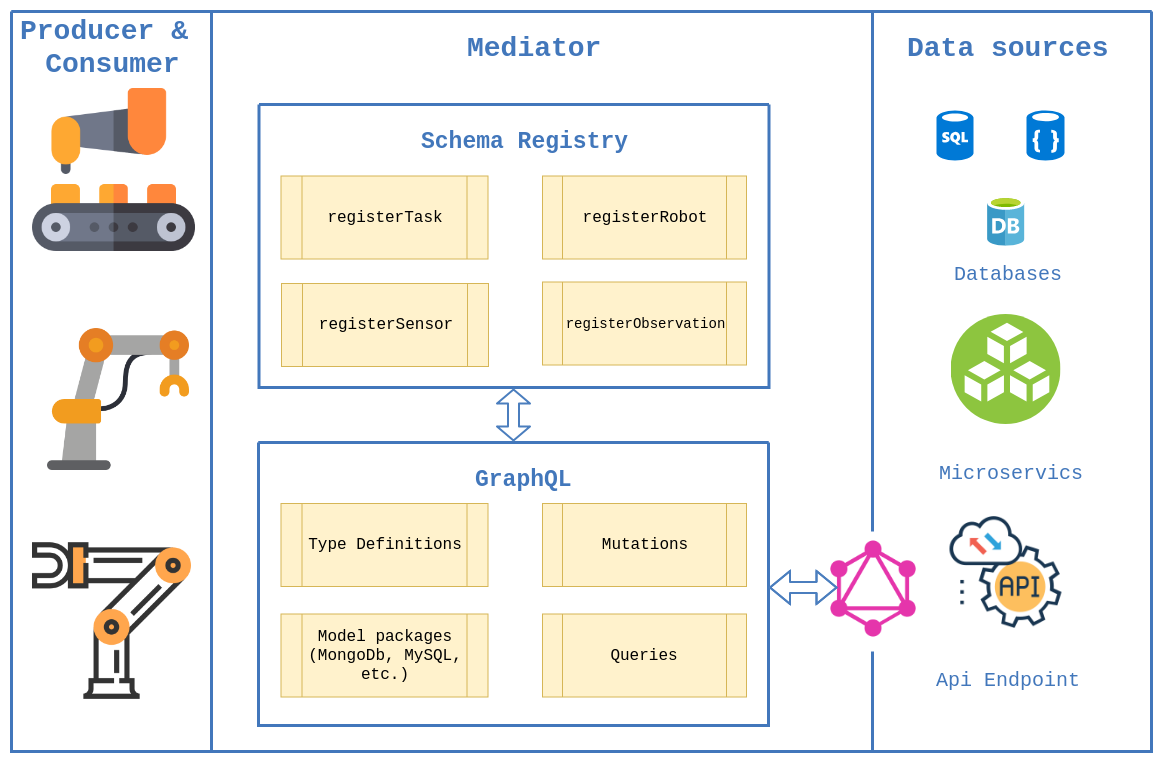
\includegraphics[scale=0.4]{./images/png/implementation/Architecture}	
			\caption{Mediator system architecture (Images used in architecture are cited here \cite{misc18} , \cite{misc17})}	
			\label{fig:architecture}	
		\end{center}
	\end{figure}
	
	
	\subsection{Mediator} 
	The essential section in the architecture is the mediator component considering it manages most of the interactions between consumer/producer and data sources. Mediator component again divided into subcomponents called Schema Registry and GraphQL mediation.  These two components are developed as individually isolated docker containers for modular and portability reasons. Each docker container runs on its own configuration and a small alpine Linux as the base image. The alpine base image is chosen for various reasons as follows, 
	
	\begin{enumerate}
		\item Usually, Alpine flavored images are small in size which in turn shrinks the container size. For example, Fedora version 5 base image size is 231MB, CentOS 7 base image size is 193MB, Ubuntu 16.04 base image size is 118MB and Alpine 3.6 base image size is only 3.98 MB \cite{misc16}. We can see that the Alpine base image is more than 90\% smaller than other flavors. 
		\item Contain only the basic functionalities without GUI components. 
		\item Faster container creation and boot time. For example, Debian based container creation took around 28 seconds and Alpine based container creation took only 5.6 seconds \cite{misc16}. Note that, this comparison is performed without cache.
		\item Safe and secure. Fewer risks of attack if there are less number of packages and libraries available in the base system. A few years ago,  a severe vulnerability was exploited called "ShellShock" which give access to hackers to execute bash commands on the server over an HTTP request. Alpine is safe from "ShellShock" attack because it does not have bash installed by default \cite{misc16}.	
	\end{enumerate}
	
	\subsubsection{Schema registry} \label{subsubsection:schema_registry}
	
	Schema registry is the entry point for registering the tasks, robots, and sensors as a relational model. This step is mandatory to let the mediator component knows the relationship between the entities and also the exact structure of sensor data. This structure of sensor data is represented in the form of JSON schema which is used for GraphQL schema transformation which is discussed in registering observation section. 
	
	Schema registry itself is an individual docker container which runs "express" server to provide the schema registration service. Express.js is a modular light-weight web application framework developed to run with Node.js platform. In the schema registry, the express server opens an endpoint for the entity and schema registration.
	
	Entity and schema registration is a sequential step by step process to store the task, robot and sensor registration, and creating new observation buckets in the real database. All the entities and their attributes are defined as follows,
	
	\textbf{Task}- A task determines the experiment which is carried out with a set of robots and sensors. 
	
	\begin{table}[!htbp]
		\begin{tabular}{|l|p{8cm}|}
			\hline
			\textbf{Attributes} & \textbf{Definitions} \\ \hline
			id & Unique UUID for each task \\ \hline
			name &  Name of the task \\ \hline
			@context &  Context for the attributes\\ \hline
			creator &  Name or id of the person who created this task\\ \hline
			creationTime &  Time of the task creation\\ \hline
			startTime & Time of the task that started\\ \hline
			endTime &  Time of the task that ended\\ \hline
			
		\end{tabular}
		\caption{Task entity attributes description}
		\label{tab:task_entity}
	\end{table}

	\textbf{Robot} - A robot entity holds the information of the robot.
	
	\begin{table}[!htbp]
		\begin{tabular}{|l|p{8cm}|}
			\hline
			\textbf{Attributes} & \textbf{Definitions} \\ \hline
			id & Unique UUID for each robot \\ \hline
			name & Name of the robot \\ \hline
			@context & Context for the attributes \\ \hline
			type & Type of the robot \\ \hline
			id & Unique identified for the robot \\ \hline
			macAddress & Mac address of the robot \\ \hline
			
		\end{tabular}
		\caption{Robot entity attributes description}
		\label{tab:robot_entity}
	\end{table}

	\textbf{Sensor} - A sensor entity defines the details of the sensor used in the robot.

	\begin{table}[!htbp]
		\begin{tabular}{|l|p{12cm}|}
			\hline
			\textbf{Attributes} & \textbf{Definitions} \\ \hline
			id & Unique UUID for each sensor \\ \hline
			name & Name of the sensor \\ \hline
			@context & Context for the attributes \\ \hline
			type & Type of the sensor \\ \hline
			description & Short description of the sensor \\ \hline
			measures & What physical characteristic that the sensor measures from the environment \\ \hline
			valueSchema & A JSON Schema represents the structure of the data that this sensor will generate. \\ \hline
			unit & Unit for the measured observation\\ \hline
			meta & Meta attribute allow users to add any additional information about the sensor which is missing in the given attribute list.\\ \hline
			
		\end{tabular}
		\caption{Sensor entity attributes description}
		\label{tab:sensor_entity}
	\end{table}
	
	\newpage
	\textbf{TaskRobotSensor} - TaskRobotSensor entity doesn't store any information about other entities; instead it stores only the relationship between a task, robot, and senor. We introduce this pivot relation because we need a way to relate entities in non-relational databases too. This type of table is called a pivot table. Pivot tables can be used to represent the relationships between different entities stores in other tables/collections. Additionally, pivot tables can have their own attributes, and this TaskRobotSensor pivot entity has startTime and endTime as additional properties to identify at what time a robot has joined the task, or when a sensor is attached with this robot. 
	
	\begin{table}[!htbp]
		\begin{tabular}{|l|p{12cm}|}
			\hline
			\textbf{Attributes} & \textbf{Definitions} \\ \hline

			id &  Unique UUID for each TaskRobotSensor relation \\ \hline			
			task & Unique task UUID \\ \hline
			robot & Unique robot UUID \\ \hline
			sensor & Unique sensor UUID \\ \hline
			startTime & Time shows when this relation has been made \\ \hline
			endTime & Time shows when this relation has been ended (if this value is not provided, then the Task endTime will be considered as TaskRobotSensor endTime) \\ \hline
			
		\end{tabular}
		\caption{TaskRobotSensor entity attributes description}
		\label{tab:TaskRobotSensor}
	\end{table}

	\textbf{Observation} - Observation is a generic entity, and it can be extended to any sensor that generates data. For each new sensor entity, a new observation bucket will be created in the name senor. The naming convention of each bucket should be unique to avoid conflicts, and the name is derived from the sensor name, and "Observation" keyword will be attached at the end. For example, consider we create a new observation bucket in MongoDB for the sensor "command velocity". Schema registry component will create a new collection in MongoDB in the name of "CommandVelocityObservation". Multiple robots are allowed to have observation buckets with the same name, but a single robot should not have duplicate observation buckets. Each observation contains the real observed data from the sensor and also the relations with the task, robot, and sensor.

	\begin{table}[!htbp]
		\begin{tabular}{|l|p{12cm}|}
			\hline
			\textbf{Attributes} & \textbf{Definitions} \\ \hline
			
				id & Unique UUID for each observation \\ \hline
				name & Name of the observation \\ \hline
				@context & Context for the attributes \\ \hline
				featureOfInterest & Tells the important feature from the observed value \\ \hline
				value & Data generated by the sensor \\ \hline
				task & Unique task UUID \\ \hline
				robot & Unique robot UUID \\ \hline
				sensor & Unique sensor UUID \\ \hline
				phenomenonTime & Time of observation created by the sensor \\ \hline
				resultTime & Time of observation stored in the database \\ \hline
			
		\end{tabular}
		\caption{Generic observation entity attributes description}
		\label{tab:observation}
	\end{table}

	\subsubsection{Schema registration workflow}
	Figure \ref{fig:schema_registration} shows the broad outline of schema registration workflow and also the essential subtasks such as registerTask,  registerRobot, and registerSensor. Schema registration endpoint "/schema-registry" allows users or robots to POST a complete schema registration over HTTP request and the schema configuration [footnote - schema configuration is included in the appendix] contains the task information, array of robot objects and each robot object consists of an array of sensor object. After the starting point in the flow chart, the parse schema config function starts parsing the given schema configuration and checks the validity of the configuration. If the configuration is valid, then execution moves to the next step and checks for a task configuration. If task config exists, then it proceeds to the very first subtask called registerTask and all the subtasks are briefly outlined in section [Workflow of subtasks]. If there is no task configuration or the task registration is unsuccessful, then the execution will be aborted.  After the successful task registration, the process starts iterating the robots array. 
	
	For each robot in the array, the system checks whether it is a new robot or existing one. For existing robots user gives the UUID of the robot, and for new robots, the system expects complete information about the robot as mentioned in the robot entity section. If the robot information is available, then the operation proceeds to the registerRobot subtask. If the subtask is not successful, then the system will abort the execution, else it starts iterates the sensor list which is attached to the robot information. Like new robot check, the system checks whether the given sensor contains an already registered UUID or new sensor information. If it is a new sensor, then the system proceeds to the last subtask called registerSensor. 
	
	In any case, after entity registration failure, the system will abort the schema registration execution. However, this workflow can be configured in such a way that, ignore the registration failures and continue the execution until the end of the schema config. After each sensor registration, the system verifies whether the current sensor is the last item in the sensors array or not. If not, then the loop continues until the last sensor in the array, else it checks whether the current robot is the last item in the robots array. If not, then the loop continues until the last robot in the array.  If the system finishes the last robot in the array, then the system stops the execution with a success flag. Later, an HTTP response will be sent back to the user/robot with the status of the schema registration and additional messages if required.
	
	\begin{figure}[!htbp] 
		\begin{center}
			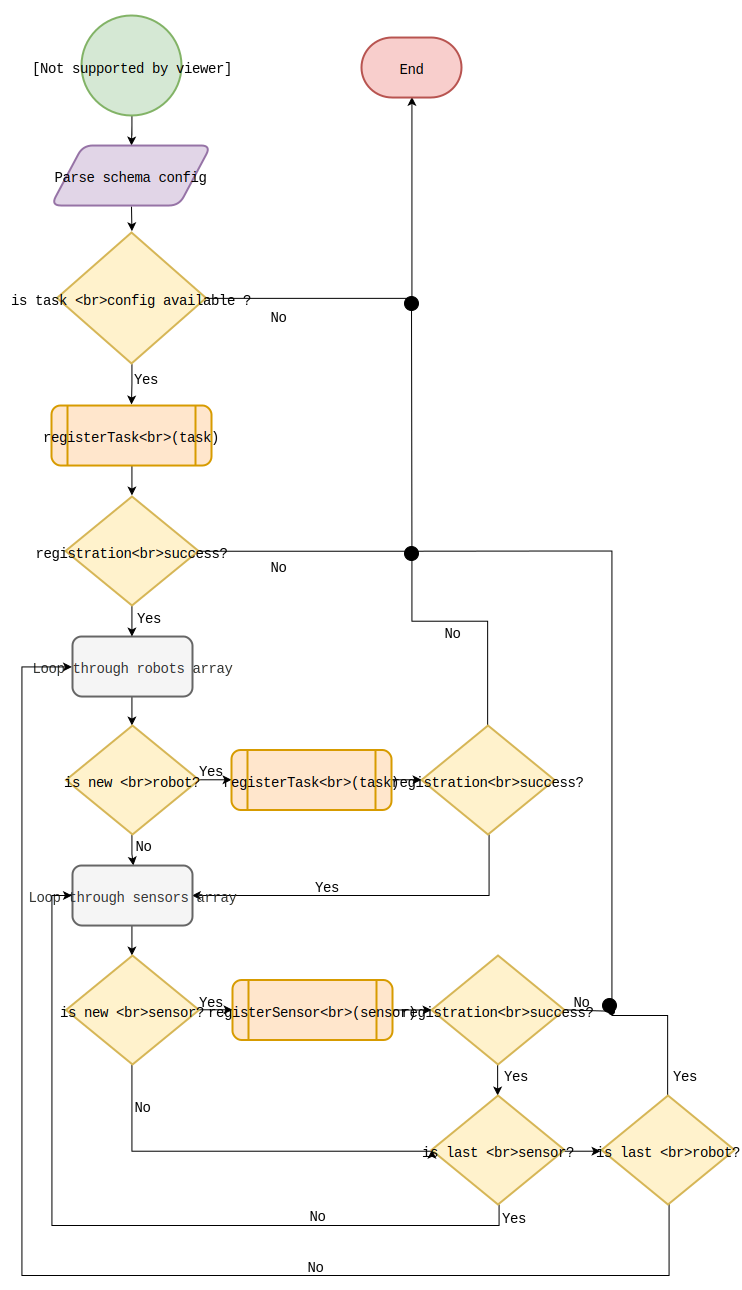
\includegraphics[scale=0.5]{./images/png/implementation/schema_registration}	
			\caption{Detailed schema registration work flow}	
			\label{fig:schema_registration}	
		\end{center}
	\end{figure}

	\subsubsection{Workflow of subtasks in schema registration}
	
	Major schema registration consists of three subtasks called registerTask, registerRobot, and registerSensor. registerTask \ref{subfig-1:task_creation} and registerRobot \ref{subfig-2:robot_creation} subtasks execution follows a similar workflow but for two different entities. At first, the system checks for the valid task/robot configuration and DB configuration respectively. If it fails, then the system aborts the execution, else system creates task/robot record in the appropriate databases. But, the system should identify the specific databases and additional information beforehand. This database entity mapping is done with the help of media config file, and it is explained in section [Entity database mapping].
	The last subtask called registerSensors \ref{subfig-3:sensor_creation} follows the similar workflow like registerTask and registerRobot, however, after each successful sensor record creation, the system should carry out another major subtask called "Create observation bucket" which is explained in section \ref{subsubsection:observation_bucket}.
	
	\begin{figure*}[!htbp]
     \subfloat[Workflow that represents creation of new task entity during schema registration\label{subfig-1:task_creation}]{%
			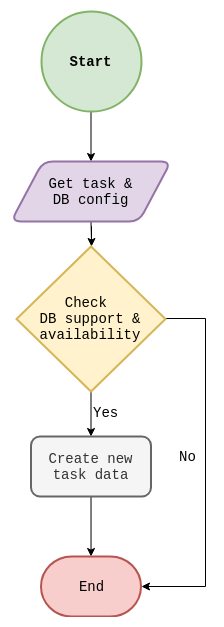
\includegraphics[scale=0.5]{./images/png/implementation/task_creation}
		}
		\hfill
		\subfloat[Workflow that represents creation of new robot entity during schema registration\label{subfig-2:robot_creation}]{%
			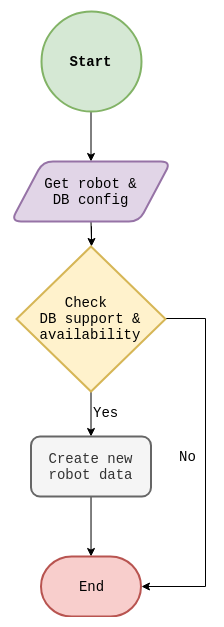
\includegraphics[scale=0.5]{./images/png/implementation/robot_creation}
		}
			\hfill
	\subfloat[Workflow that represents creation of new sensor entity during schema registration\label{subfig-3:sensor_creation}]{%
		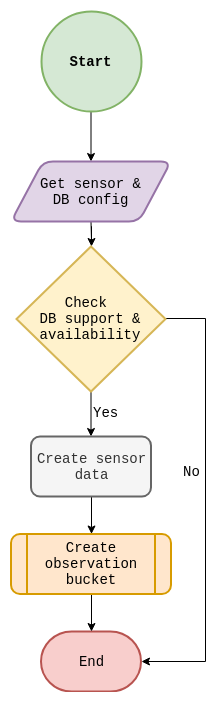
\includegraphics[scale=0.5]{./images/png/implementation/sensor_creation}
	}
		\caption{Decomposition of major entities creation work flow}
		\label{fig:dummy}
	\end{figure*}
	\newpage
	\subsubsection{Observation bucket creation workflow} \label{subsubsection:observation_bucket}
	This module includes a series of actions that need to be performed to make sure the new observation buckets are available after the creation of the new sensor, in all possible databases/data-sources which is defined in mediator config file. The naming convention for new buckets is already discussed in the "Observation" topic under section \ref{subsubsection:schema_registry}. Once after successfully created the buckets, schema registry should update the changes to GraphQL mediation component (second docker container). Three things need to be updated in the GraphQL mediation component as follows,
	
	\begin{enumerate}
		\item GraphQL type definition - GraphQL frameworks identify all the data attribute types via type definition file. So we need to update this type definition with the newly created sensor output structure. Each sensor object consists of an attribute called "valueSchema" which shows how the observation data will look like from this specific sensor. This schema is nothing but a JSON Schema file with all attribute types and constraints imposed on them. This JSON Schema to GraphQL schema conversion is done by a transformer module which is explained in section \ref{subsubsection:jsonschema_graphqlschema}.
		
		\item GraphQL queries - GraphQL queries consist of all possible queries that can be executed on the GraphQL mediation server. Here, the system should update new queries to fetch the new observation data from various buckets.
		
		\item GraphQL mutations - GraphQL mutation helps users to create new records in the database. But, it is not mandatory to create records via the GraphQL mediation component, because robots can generate the data and store them directly to their local database instances. Later the person who wants to make fault diagnosis or to debug, they can configure the DB's with the mediator and fetch data via GraphQL queries.
	\end{enumerate}
	\newpage
	\begin{figure}[!htbp] 
		\begin{center}
			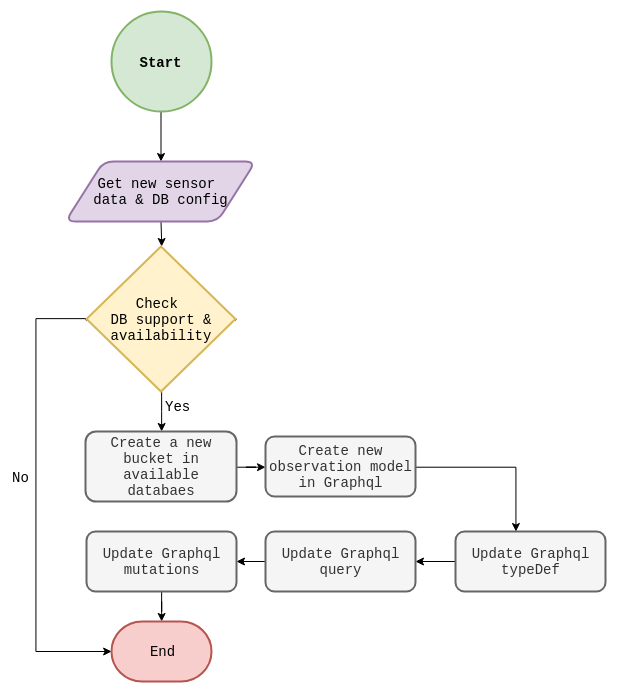
\includegraphics[scale=0.5]{./images/png/implementation/observation_creation}	
			\caption{Observation bucket creation work flow}	
			\label{fig:observation_creation}	
		\end{center}
	\end{figure}
	
	\subsubsection{Entity database mapping}
	For creating new tasks, robots, and sensors data during schema registration, schema registry should have an idea where to create these records. We propose an entity database mapping strategy to identify the databases for each entity. To make it more flexible, we assign each entity to a database name, and the corresponding database configuration is described in the same config file under "db" attribute which is shown in figure \ref{fig:entity_db_mapping}. The "db" attribute contains a list of db configuration and the attributes in each db object is explained in table \ref{tab:db_attribute_desc}. 
	
	\begin{table}[h!]
		\begin{tabular}{|l|p{12cm}|}
			\hline
			\textbf{Attributes} & \textbf{Definitions} \\ \hline
			
			name & Unique name for each database and this name is used to identify the database configuration in the mediator system internally. Don't confuse this attribute with "dbName". \\ \hline
			type & Type of the database. Currently, the mediator system supports mongodb and mysql. \\ \hline
			url & URL to access the database. \\ \hline
			dbName & The actual name of the database. \\ \hline
			userName & Username to access the database (not mandatory). \\ \hline
			password & Password to access the database (not mandatory). \\ \hline
			
		\end{tabular}
		\caption{Single db object attributes description}
		\label{tab:db_attribute_desc}
	\end{table}
	
	
	In the given example \ref{fig:entity_db_mapping}, under "entityDBMapping" attribute, each entity is mapped to a name of the database which is described under "db" attribute. The "observations" entity consists of an array of database names, because the sensor generated data may be available in multiple robots/datasources. With the help of this mapping, the schema registry gets the information about where to create new records. This same mediator config file is also shared with GraphQL mediation component.
	
	\begin{figure}[!htbp] 
		\begin{center}
			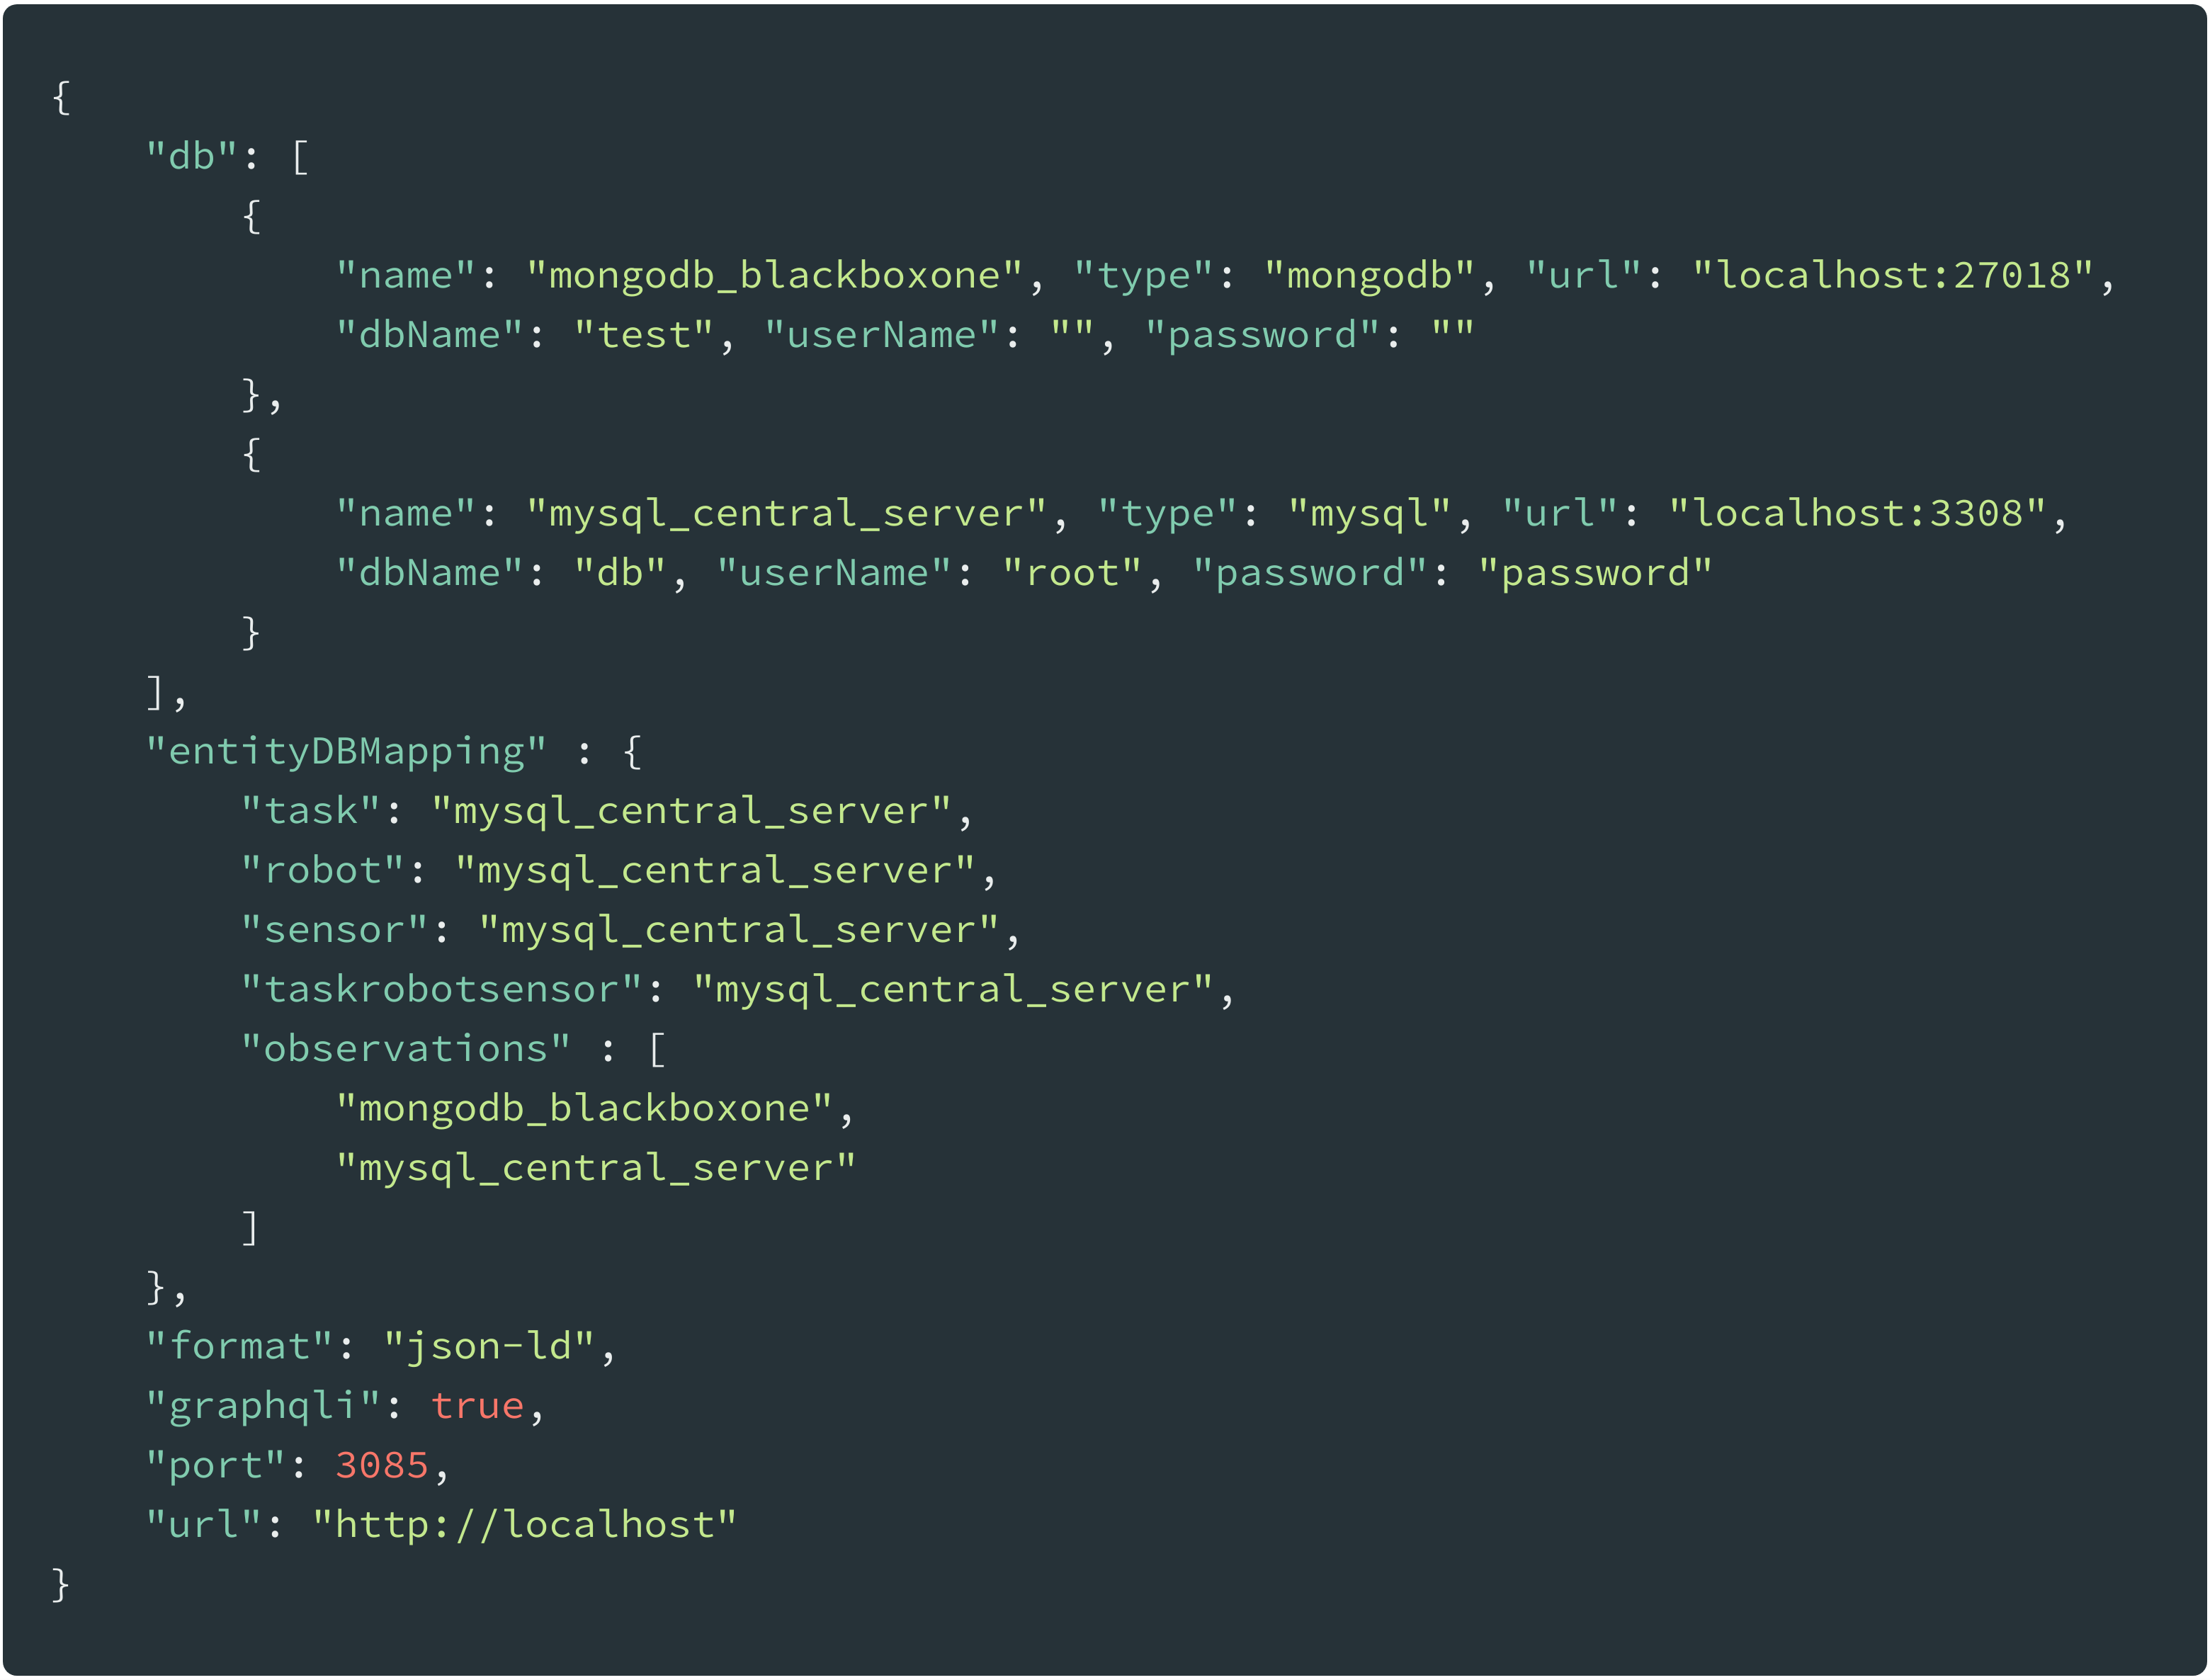
\includegraphics[scale=0.1]{./images/png/implementation/entity_db_mapping}	
			\caption{Entity database mapping representation in mediator config file}	
			\label{fig:entity_db_mapping}	
		\end{center}
	\end{figure}

	\subsubsection{JSON Schema to GraphQL Schema transformation} \label{subsubsection:jsonschema_graphqlschema}
	
	The mediator component is using GraphQL framework as a base to utilize the features \ref{sec:graphql_falcor} offered by GraphQL out of the box. GraphQL needs a type definition document to work on even before starting the server.  Through schema registration, user/robot provide a JSON Schema which represents how the sensor data would look like in the observation bucket.  JSON Schema \ref{sec:json_schema} is a well known schematic representation for data, so we decided to use this as a generic data schema format to represent the sensor observation structure. Later the JSON Schema to GraphQL transformation module in "Schema registry" component translates the JSON Schema to GraphQL type definition through a series of steps as shown in the figure \ref{fig:jsonscema_to_graphql}. There are three steps involved in the transformation as follows,
	
	\begin{enumerate}
		\item Get the JSON Schema from the valueSchema attribute in sensor object and validate the schema structure. After validation, pass the JSON Schema to the next step.
		\item In this step, we use an open source library  "djvi \footnote{ \url{https://github.com/korzio/djvi}}" to generate the model prototype from the JSON Schema. This model prototype resembles precisely the same as the observation that will be generated by the sensor in the future.
		\item Finally, based on this model prototype, the schema registry system creates an equivalent GraphQL schema (type definition), and the new schema is appended to the current GraphQL type definition file.
	\end{enumerate}
	
	\begin{figure}[!htbp] 
		\begin{center}
			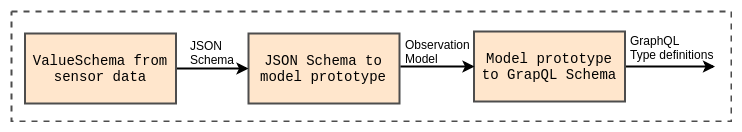
\includegraphics[scale=0.5]{./images/png/implementation/jsonscema_to_graphql}	
			\caption{Process of JSON Schema to GraphQL Schema (type definition) conversion}	
			\label{fig:jsonscema_to_graphql}	
		\end{center}
	\end{figure}

	In the end, GraphQL will consume the new updated file, and users/robots can write/read new sensor observations from different datasources.
	
	\subsubsection{GraphQL mediation}
	Mediation component is a separate docker container which is built based on express server and Apollo GraphQL wrapper. Apollo GraphQL wrapper is implemented based on facebook GraphQL specification and designed their system as a wrapper to run on top of the express server. To run the Apollo GraphQL server, it requires four mandatory modules such as,
	\begin{enumerate}
		\item Type definitions - It consists of data type definition for all the entities which users are going to query or write into the database. In the context of our research work, this module consists of schemas for Task, Robot, Sensor, TaskRobotSensor and all type of Observations. Additionally, it may have the queries and mutations outline but not their definition.
		\item Mutations - This module consists of required functions to receive the incoming data and write/update in the database.
		\item Queries - This module includes necessary services to fetch data from the database.  
		\item Model packages - This is a custom module which comprises of model definitions of each entity for all the supported databases. Currently GraphQL mediation component supports MongoDB and MySQL. The system uses two open-source libraries called "mongoose \footnote{ \url{https://github.com/Automattic/mongoose}}" and "sequelize \footnote{ \url{https://github.com/sequelize/sequelize}}" to make the connection and communication between the GraphQL mediation component and the respective databases. Both modules are designed to follow ORM (Object Relation Mapping) pattern to let developers write their code in a class structure which is convenient and easy to maintain the code base. The mongoose module targets only MongoDB and sequelize can be used to interact with Postgres, MySQL, MariaDB, SQLite, and Microsoft SQL Server.		
	\end{enumerate}

	\subsubsection{Connection pool management} 
	Both the schema registry and GraphQL mediation components initiate their database connection pool before the server starts. The system creates different database connections based on the "db" configurations mentioned in the mediator config file \ref{fig:entity_db_mapping} . And this database connection pool is shared across the component such that other services like queries and mutations can use it to read or write data into databases.
	
	\subsection{Data sources} 
	The rightmost block in the architecture \ref{fig:architecture} represents the data sources. A data source can be any databases, microservices, or an API endpoint. GraphQL component serves as a bridge between the robot and data sources. In the current work, we used only MongoDB and MySQL as data sources. However, the mediator can be extended to support other databases with little modifications in the GraphQL Queries and Mutations module.
	
	\subsection{Summary}
	In the above sections, the three major subdivisions of the mediator architecture and their responsibilities are explained elaborately. And the next section evaluates the current mediator design with the requirements and existing black box data storage design.
	
\end{document}
